%!TEX encoding = UTF-8 Unicode
%!TEX root = ../compendium.tex

\chapter{Integrerad utvecklingsmiljö}\label{appendix:ide}

\section{Vad är en integrerad utvecklingsmiljö?}

En integrerad utvecklingsmiljö \Eng{integrated development environment, IDE} samlar ett flertal verktyg, inklusive en avancerad \textbf{editor} (se appendix \ref{appendix:edit}), för att skapa, köra och testa program. Det finns flera utvecklingsmiljöer att välja mellan, som kan användas för både Scala och Java.

En IDE ger stöd för auto-komplettering \Eng{auto completion} där tillgängliga metoder visas i en lista och resten av ett namn kan fyllas efter att du skrivit de första bokstäverna i namnet. En IDE kan hjälpa dig med formattering och även skapa skelettkod utifrån \textbf{kodmallar} \Eng{code templates}. Med \textbf{felindikering} \Eng{error highlighting} får du understrykning av vissa fel direkt i koden och ibland kan du även få hjälp med förslag på åtgärder för att rätta till enkla fel. Funktioner för \textbf{avlusning} \Eng{debugging} hjälper dig att felsöka medan du kör din kod. Med funktioner för \textbf{omstrukturering} \Eng{refactoring} av kod får du hjälp av editorn i samarbete med kompilatorn att göra omfattande strukturförändringar i många kodfiler samtidigt, t.ex. namnbyten med hänsyn taget till synlighetsregler.  

Alla dessa avancerade funktioner kan öka produktiviteten avsevärt, men samtidigt tar de tid att lära sig och en IDE kan kräva mycket datorkraft och viss väntetid jämfört med en vanlig, fristående editor. I början kan all funktionalitet upplevas som överväldigande och det kan vara svårt att hitta i alla menyer och inställningar. Ska man bara skriva ett litet, enkelt program, eller göra några mindre ändringar, är det många som föredrar en fristående, snabbstartad kodeditor före en fullfjädrad, tungrodd IDE. Å andra sidan kan en IDE hjälpa till att upptäcka vad som finns i ett api och autokompletteringsfunktionen hjälpa stort när man upptäcker och experimenterar med en okänd kodmassa.


\section{Kojo}\label{appendix:kojo}

\subsection{Installera Kojo}

\href{http://www.kogics.net/kojo-download}{www.kogics.net/kojo-download}

\subsection{Använda Kojo}

\begin{table}[h]
\caption{Några av sköldpaddans funktioner. Se även \href{http://lth.se/programmera}{lth.se/programmera}}
\vspace{1em}\small
\begin{tabular}{lll}
\emph{Svenska} & \emph{Engelska} & \emph{Vad händer?}\\ \hline
\tt fram     & \tt forward     & Paddan går 25 steg frammåt.           \\
\tt fram(50) & \tt forward(50) & Paddan går 50 steg frammåt.           \\
\tt höger    & \tt right       & Paddan vrider sig 90 grader åt höger. \\
\code+upprepa(10){???}+ & \code+repeat(10){???}+  & Repetition av ??? 10 gånger. \\
\end{tabular}
\end{table}

\noindent Koden för den svenska paddans api finns här:
\href{https://bitbucket.org/lalit\_pant/kojo/src/tip/src/main/scala/net/kogics/kojo/lite/i18n/svInit.scala?at=default\&fileviewer=file-view-default\#svInit.scala-26}{bitbucket.org/lalit\_pant/kojo/}

\section{Eclipse och ScalaIDE}\label{appendix:ide:eclipse}

\subsection{Installera Eclipse och ScalaIDE}\label{appendix:ide:eclipse:install}

\subsection{Använda Eclipse och ScalaIDE}\label{appendix:ide:eclipse:use}

\subsubsection{Ladda ner och importera projekt från kursens workspace}

TODO: skriv mer här

\begin{itemize}
\item Ladda ner kursens workspace här: \url{http://cs.lth.se/pgk/workspace}
\item Packa upp filen på lämpligt ställe.
\item Starta Eclipse med ScalaIDE-plugin (för installation se \ref{appendix:ide:eclipse:install}).
\item Bläddra till biblioteket du nyss packade upp, ungefär som i \ref{fig:eclipse:ide:open}
\begin{figure}[H]
\centering
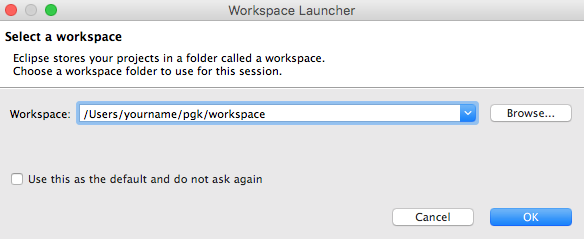
\includegraphics[width=0.7\textwidth]{../img/pirates/selectws.png}
\caption { \emph{Öppna workspace:} Bläddra fram till kursens workspace och klicka {\bf OK. }}
\label{fig:eclipse:ide:open}
\end{figure}

\item Gå vidare från startskärmen genom att välja {\bf Workspace}, se Fig.\ref{fig:eclipse:ide:selectws}.
\begin{figure}[H]
\centering
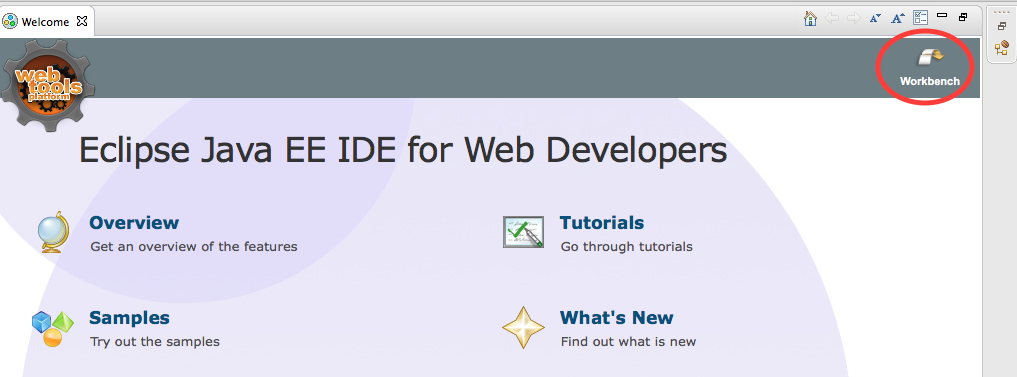
\includegraphics[width=0.7\textwidth]{../img/pirates/selectws2.png} \\

\caption {Välj {\bf workspace}.}
\label{fig:eclipse:ide:selectws}
\end{figure}

\item Uppe till höger ser du vilken \emph{vy} du har. I Eclipse kommer vi växla mellan Scala, Java och debug-vyer. Dessa läggs till via listan som nås genom den fönsterliknande ikonen enligt Fig.~\ref{fig:eclipse:ide:changeview}. Du ska ha {\bf Scala} igång.

\begin{figure}[H]
\centering
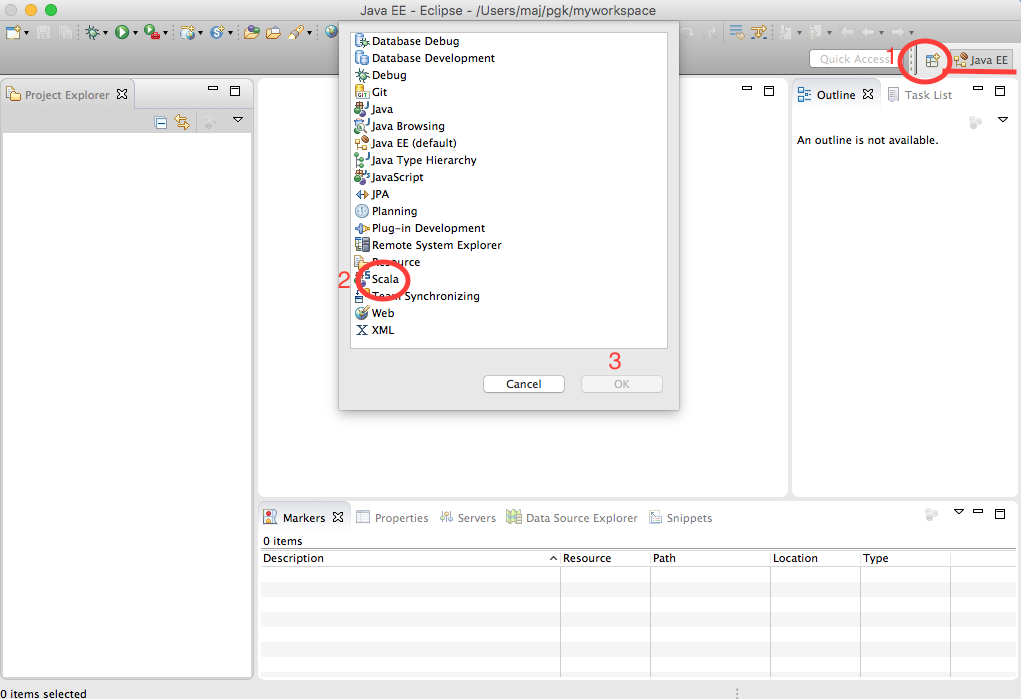
\includegraphics[width=0.7\textwidth]{../img/pirates/selectscala.png} 

\caption {Lägg till vyer från listan med installerade plugin.}
\label{fig:eclipse:ide:changeview}
\end{figure}

\item Högerklicka i {\bf Project Explorer} och välj {\bf New} -> {\bf Scala Project}, se Fig.~\ref{fig:eclipse:ide:createproject}. Importera existerande project genom att genom att avmarkera \emph{Use default location} och bläddra till katalogen för respektive laboration och sen {\bf Finish}, se exempel i Fig.~\ref{fig:eclipse:ide:import} (namnet sätts automatiskt). Du kan också skapa nya projekt genom att ange ett projektnamn direkt och sen klicka {\bf Finish} enligt Fig.~\ref{fig:eclipse:ide:newproject}.

\begin{figure}[H]
\centering
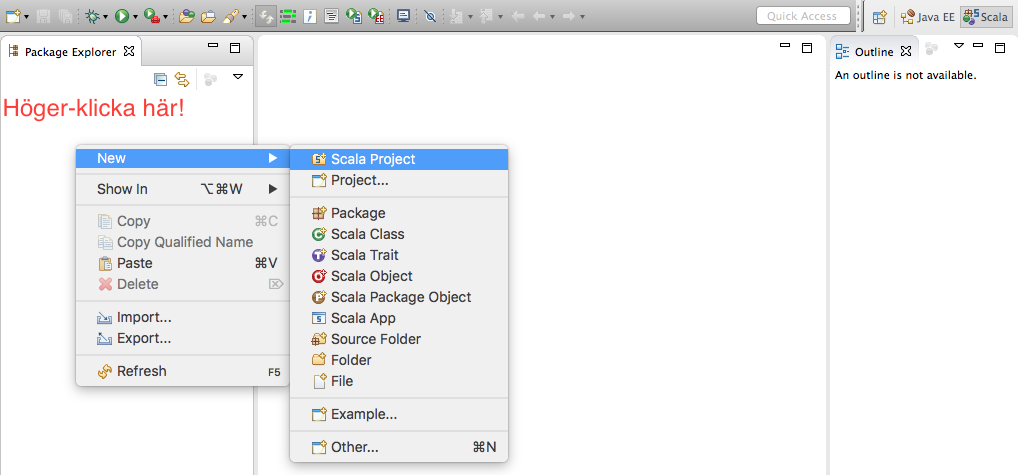
\includegraphics[width=0.7\textwidth]{../img/pirates/createproject.png} 

\caption {Välj att {\bf Scala Project} i menyerna.}
\label{fig:eclipse:ide:createproject}
\end{figure}
\begin{figure}[H]
\centering
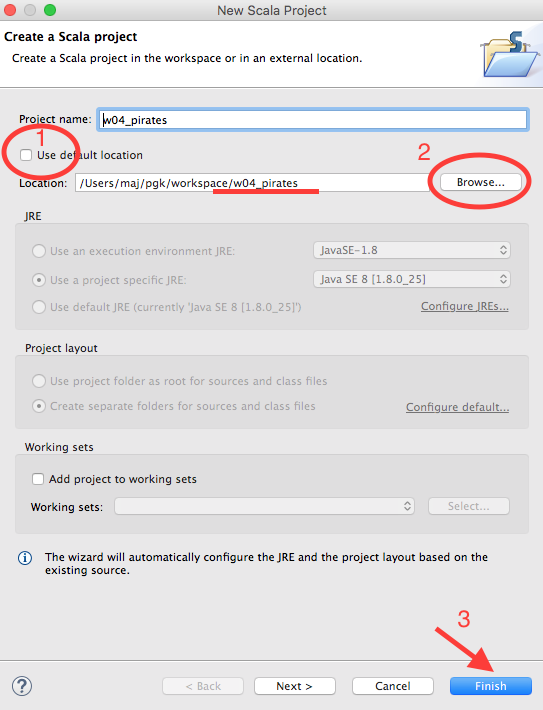
\includegraphics[width=0.5\textwidth]{../img/pirates/importproject.png} 

\caption {Importera existerande projekt genom att ange sökvägen.}
\label{fig:eclipse:ide:import}
\end{figure}

\begin{figure}[H]
\centering
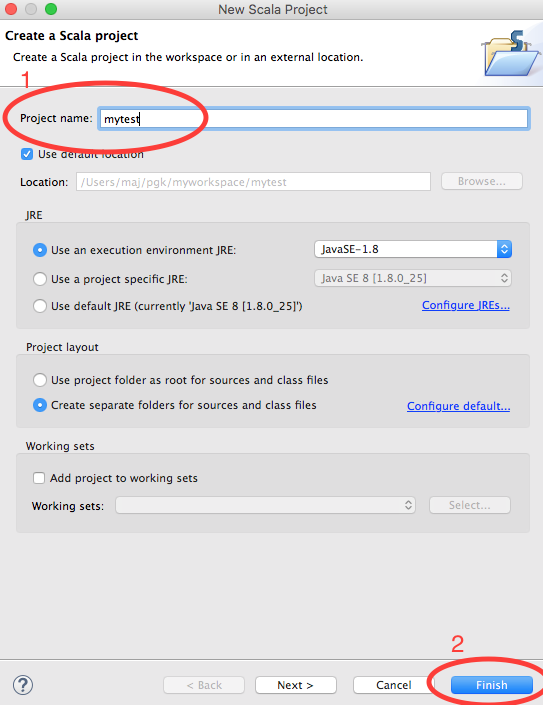
\includegraphics[width=0.5\textwidth]{../img/pirates/nameproject.png} 

\caption {Skapa ett nytt projekt genom att ange namn.}
\label{fig:eclipse:ide:newproject}
\end{figure}


\item Du skapar nya klasser och objekt på liknande sätt, genom att högerklicka och välja {\bf New}, se exempel i Fig.~\ref{fig:eclipse:ide:createobject}


\begin{figure}[H]
\centering
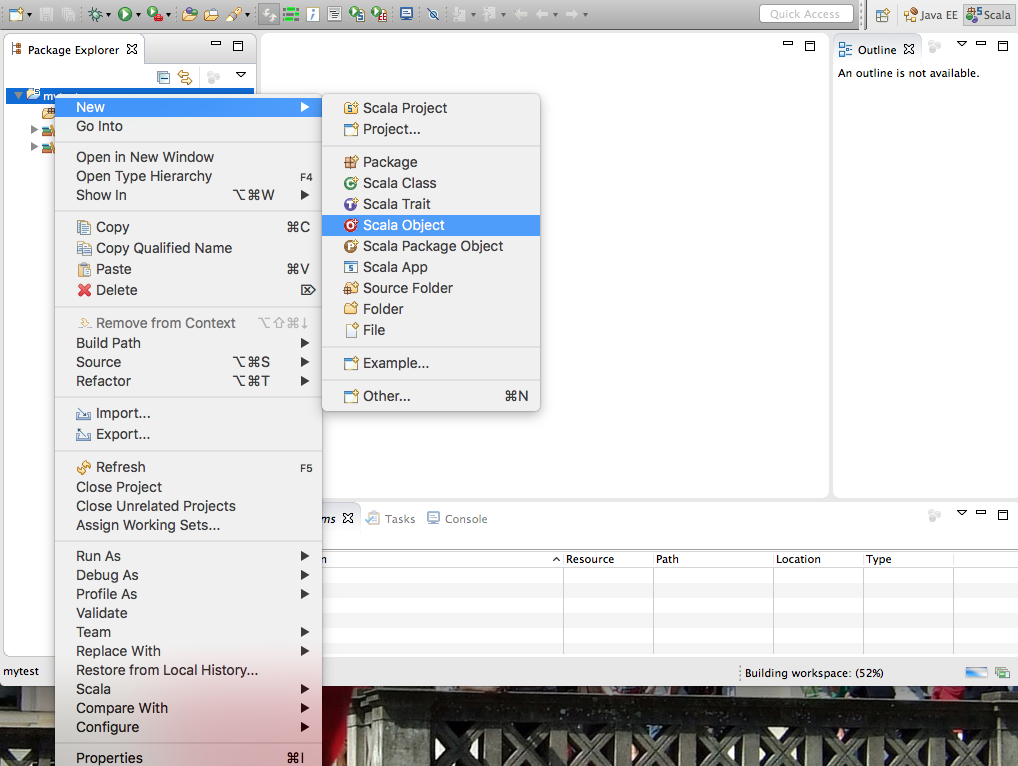
\includegraphics[width=0.7\textwidth]{../img/pirates/createobject.png} 
\caption {Skapa ett nytt objekt via menyerna.}
\label{fig:eclipse:ide:createobject}
\end{figure}

\item Skriv ett main-program och exekvera det genom att markera klassen i {\bf Project Explorer} och sen klicka på den gröna pilen. Utskrifter kommer till konsolen längst ner. 

\begin{figure}[H]
\centering
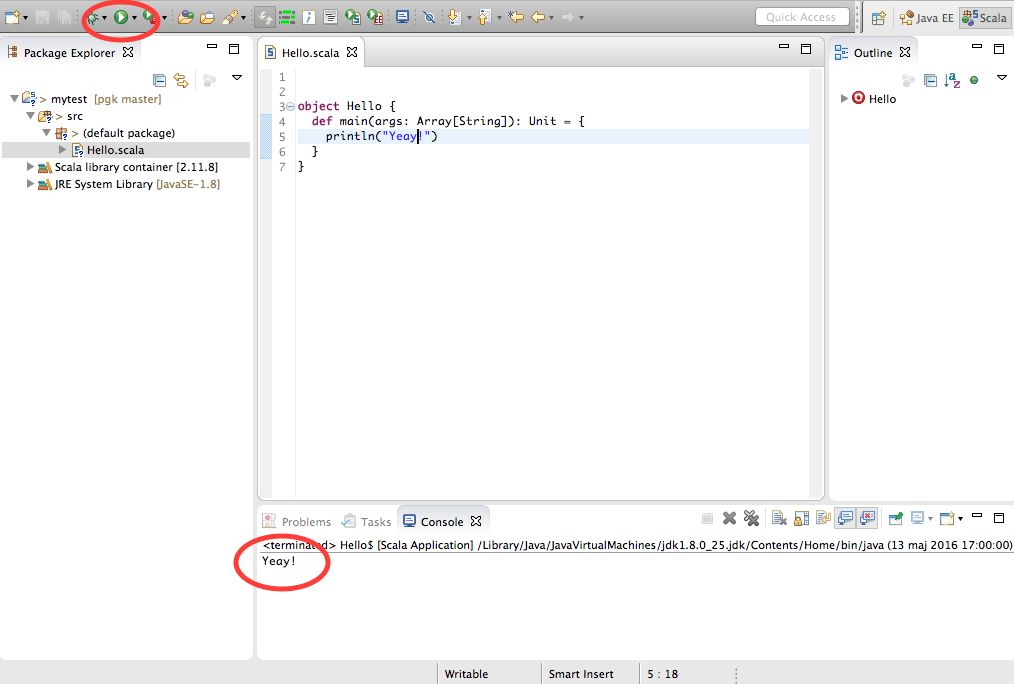
\includegraphics[width=0.7\textwidth]{../img/pirates/exekvera.png} 
\caption {Exekvera med den gröna pilen.}
\label{fig:eclipse:ide:exec}
\end{figure}
\end{itemize}



